% !TEX root = NotesDeCours.tex




%%%%%%%%%%%%%%%%%%%%%%%%%%%%%%%%%%%%%%%%%%%%%%%%%%%%%%%%%%%%%%%%%%%%%%%%%%%%%%%%%%%%%%%%%%
\part{Ecoulements visqueux}
%\setcounter{section}{5}
%\beamer@tocsectionnumber=5\relax
\section{Ecoulements visqueux}
%%%%%%%%%%%%%%%%%%%%%%%%%%%%%%%%%%%%%%%%%%%%%%%%%%%%%%%%%%%%%%%%%%%%%%%%%%%%%%%%%%%%%%%%%%



\begin{frame}

  \color{bleu}

  \begin{flushleft}
    
    \Large
   	\bf
    
    Mécanique des fluides 

  \end{flushleft}
  
  \ligne{3} % remplace: \noindent \thickline{0.5mm}{150}

  \begin{flushright}

    \rm

    \textrm{David} \textsc{Fabre}
    
    \vspace{3mm}
    
    IMFT / UPS
    
    Département de Mécanique
    
%%    brancher@imft.fr

  \end{flushright}

\begin{picture}(110, 30)(9, -18)
  \put( 15, -22){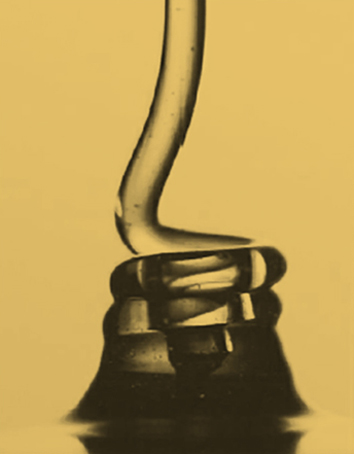
\includegraphics[height=30mm]{./Figures/miel1.jpg}}
  \put( 40, -22){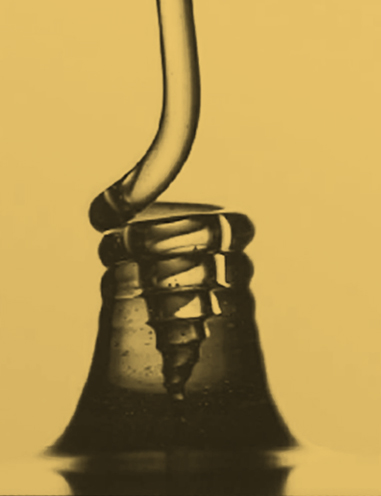
\includegraphics[height=30mm]{./Figures/miel2.jpg}}
  \put( 64.5, -22){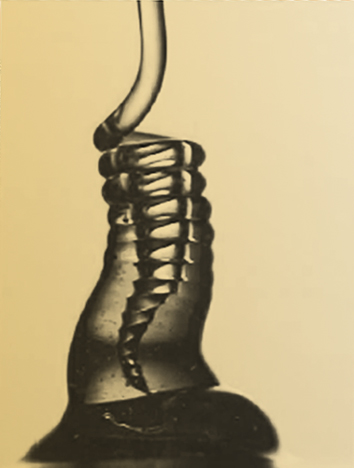
\includegraphics[height=30mm]{./Figures/miel3.jpg}}
  \put( 89, -22){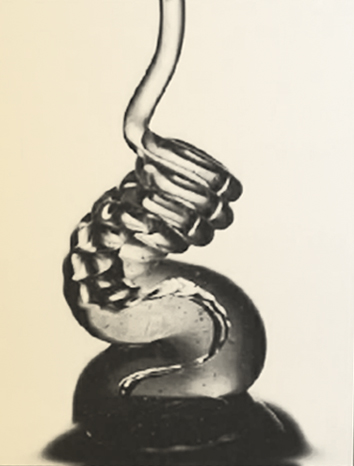
\includegraphics[height=30mm]{./Figures/miel4.jpg}}
  \put(16, -25){\color{gris} \small \rm Enroulement d'un filet de miel. Patricia ERN \copyright\ IMFT}
\end{picture}
  \vspace{7mm}
  
  \begin{flushright}
    
    \Large
   	\bf
    
    6. Ecoulements visqueux

  \end{flushright}

\end{frame}

%%%%%%%%%%%%%%%%%%%%%%%%%%%%%%%%%%%%%%%%%%%%%%%%%%%%%%%%%%%%%%%%%%%%%%%%%%%%%%%%%%%%%%%%%%
% Sommaire :
%%%%%%%%%%%%%%%%%%%%%%%%%%%%%%%%%%%%%%%%%%%%%%%%%%%%%%%%%%%%%%%%%%%%%%%%%%%%%%%%%%%%%%%%%%

%\begin{frame}{Sommaire}
%
%\small
%  
%\hspace*{2mm}
%\begin{tabular}{cc}
%		%&
%  		\begin{minipage}{62mm}
%  			\tableofcontents[firstsection=-3]
%      \vspace{15mm}
%  		\end{minipage}
%  		&   
%  		\begin{minipage}{60cm}
%		  \vspace*{-5mm}  
%  			%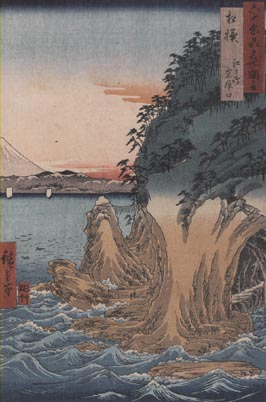
\includegraphics[width=40mm]{vagues.jpg} 
%  		\end{minipage}
%  	\end{tabular}
%
%\vspace{0mm}
%
%\end{frame}


%%%%%%%%%%%%%%%%%%%%%%%%%%%%%%%%%%%%%%%%%%%%%%%%%%%%%%%%%%%%%%%%%%%%%%%%%%%%%%%%%%%%%%%%%%

%%%%%%%%%%%%%%%%%%%%%%%%%%%%%%%%%%%%%%%%%%%%%%%%%%%%%%%%%%%%%%%%%%%%%%%%%%%%%%%%%%%%%%%%%%

%==========================================================================================
\subsection{L'approximation d'écoulement visqueux}
%=========================================================================================

%-----------------------------------------------------------------------------------------
\subsubsection{Définition}
%-----------------------------------------------------------------------------------------
\begin{frame}{Définition}
%-----------------------------------------------------------------------------------------

\small

On appelle \textcolor{rouge}{écoulement visqueux} tout écoulement pour lequel 
le mode de transport de la quantité de mouvement par diffusion visqueuse est dominant 
par rapport au tranport par advection.

\pause

\medskip

Dans ces conditions, si $U$ et $L$ désignent les échelles caractéristiques de vitesse 
et de longueur \\ de l'écoulement, le temps caractéristique de diffusion de la quantité de mouvement
$\tau_{d} = L^2/\nu$ \\
est donc beaucoup plus court que le temps d'advection 
$\tau_{a} = L/U$, soit :

\begin{equation}
  \frac{\tau_{d}}{\tau_{a}} = \frac{L^2/\nu}{L/U} \ll 1
  \quad \Rightarrow \quad
  \color{rouge} Re \equiv \frac{UL}{\nu} \ll 1
\end{equation}

o\`u $Re$ désigne le \textsl{nombre de Reynolds}.

\medskip

Les écoulements visqueux sont donc aussi appelés \textcolor{rouge}{écoulements à faible nombre de Reynolds}

\begin{center}
\begin{picture}(40, 25)(0, 0)
	\put(0, 0){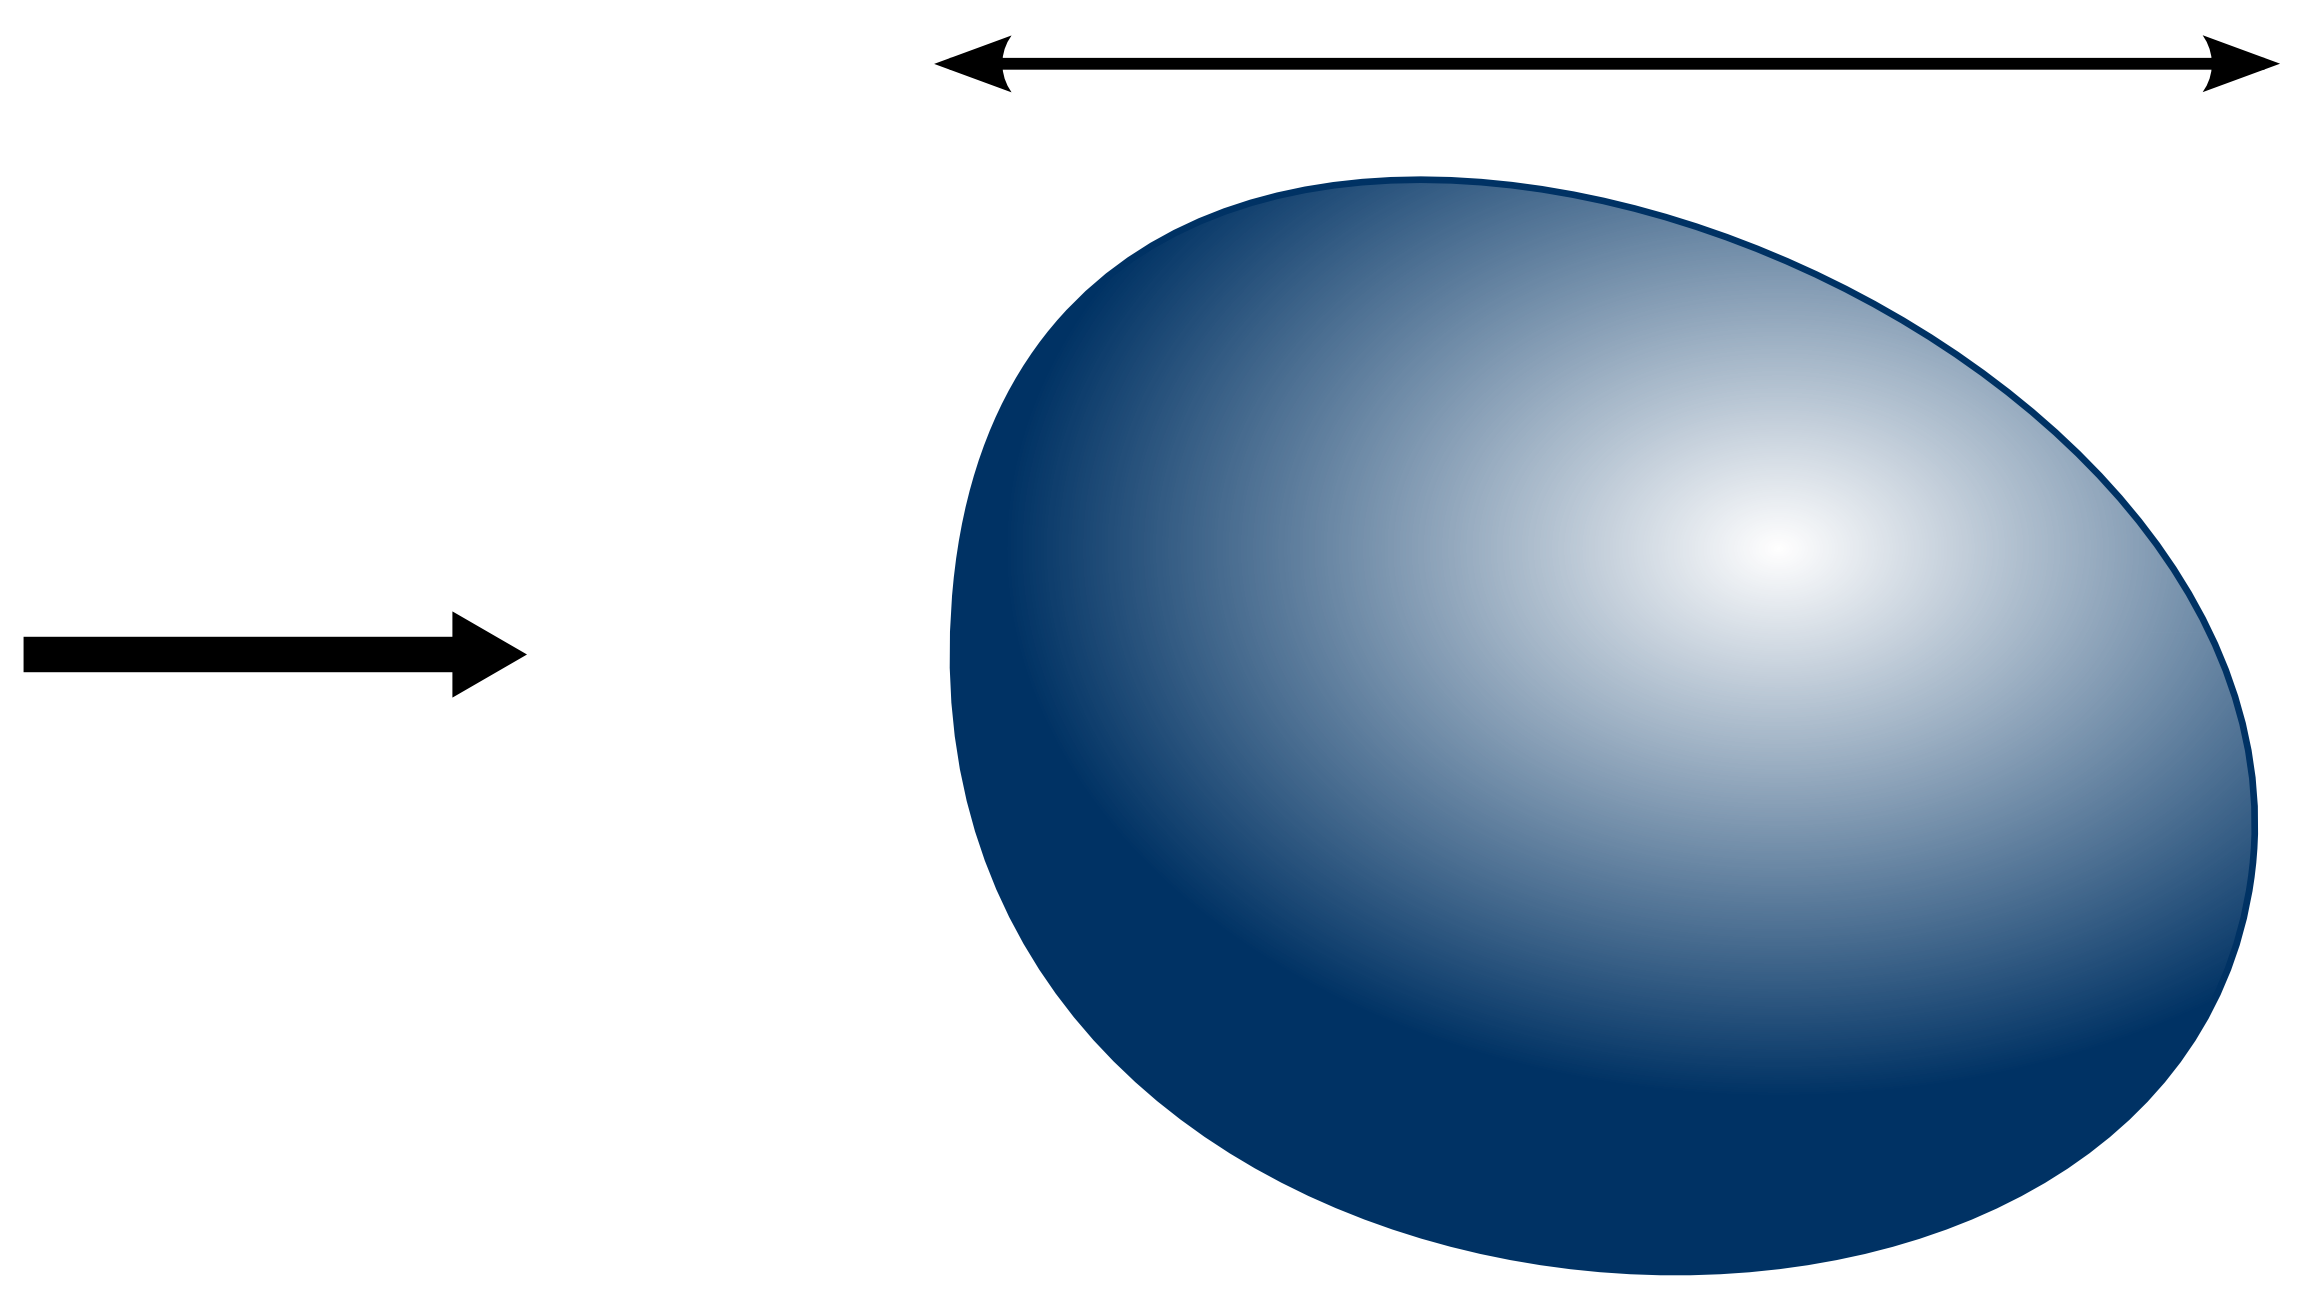
\includegraphics[width=40mm]{obstacle.png}}	
	\put(3, 13){$U$}
	\put(25, 21){\setlength{\fboxsep}{0.5mm}\colorbox{white}{$L$}}
\end{picture}
\end{center}

\vspace{0mm}

\end{frame}

%-----------------------------------------------------------------------------------------
\subsubsection{Exemples}
%-----------------------------------------------------------------------------------------
\begin{frame}{Exemples}
%-----------------------------------------------------------------------------------------

\small

Les écoulements à faible nombre de Reynolds peuvent correspondent à des écoulements 

\medskip

\begin{itemize}
\item<1->
	très \textcolor{vert}{lents} 
	\\
	Ex. glacier : $U \sim 1\ \mbox{m/jour} \sim 10^{-5}\ 
	\mbox{m/s}$; manteau terrestre : $U \sim 1\ \mbox{m/an} \sim 10^{-8}\ \mbox{m/s}$
	\medskip
\item<2->
	de fluides très \textcolor{vert}{visqueux}
	\\
	Ex. polymères, p\^ates, boues, lave : 
	$\nu \sim 10^3\ \mbox{à}\ 10^6\ \nu_{\mbox{\tiny eau}}$
	\medskip
\item<3->
 	autour de corps très \textcolor{vert}{petits} ou dans des géométries très \textcolor{vert}{confinées}
	\\
	Ex. bactéries, particules en suspension, milieux poreux : $L \sim 10^{-6}\ \mbox{m}\ \mbox{à}\ 10^{-3}\ \mbox{m}$
\end{itemize}

\vspace{25mm}

\end{frame}

%\end{document}

%==========================================================================================
\subsection{Les écoulements de Stokes}
%=========================================================================================

%-----------------------------------------------------------------------------------------
\subsubsection{Equation de Stokes}
%-----------------------------------------------------------------------------------------
\begin{frame}{Equation de Stokes}
%-----------------------------------------------------------------------------------------

\small

Considérons l'écoulement incompressible d'un fluide newtonien homogène (masse volumique uniforme), dans le champ de pesanteur (par ex.).

\pause 

\medskip

L'écoulement vérifie donc l'équation de continuité 
$\divergence \myvec{u} = 0$ et l'équation de Navier--Stokes :
\begin{equation}
  \dpdt{\myvec{u}} + (\myvec{u} \cdot \gradient) \myvec{u}
  =
  - \frac{1}{\rho} \, \gradient p + \myvec{g} 
  + \nu \, \Delta \myvec{u}
  =
  - \frac{1}{\rho} \, \gradient \hat{p} 
  + \nu \, \Delta \myvec{u}  
\end{equation}
o\`u $\hat{p} \equiv p - \rho \myvec{g} \cdot \myvec{x} = p + \rho g z$ 
est la \textcolor{vert}{pression motrice}
($z$ désigne la direction verticale ascendante).

\bigskip

\pause

Le rapport des ordres de grandeur des termes d'inertie à gauche et du terme de diffusif de droite s'écrit
\begin{equation}
  \mbox{\color{gris} [Démonstration] \; $\longrightarrow$ \;} 
  \frac{U^2/L}{\nu U/L^2} = \color{rouge}\frac{UL}{\nu} = Re \ll 1
\end{equation}

\pause
\medskip

Le terme inertiel est donc négligeable devant le terme visqueux,
d'o\`u l'\textcolor{vert}{équation de Stokes} :
\begin{equation}
  \myvec{0} = -\frac{1}{\rho} \gradient{\hat{p}} 
  + \nu \Delta \myvec{u}
  \quad \Rightarrow \quad
  \color{rouge} \gradient{\hat{p}} = \mu \Delta \myvec{u}
\end{equation}
o\`u $\mu = \rho \nu$.
Les écoulements visqueux sont donc aussi appelés 
\textcolor{vert}{écoulements de Stokes}.

\vspace{10mm}

\end{frame}

%-----------------------------------------------------------------------------------------
\subsubsection{Propriétés}
%-----------------------------------------------------------------------------------------
\begin{frame}{Propriétés}
%-----------------------------------------------------------------------------------------

\small

\begin{enumerate}

\item
L'ordre de grandeur des fluctuations de pression est donné par
\[
 \mbox{\color{gris} [Démonstration] \; $\longrightarrow$ \;} 
[ p']  / L \sim \mu U/L^2, \quad \mbox{soit} \quad
 \color{rouge}[ p' ]  \sim \mu U/L
\]
Les fluctuations de pression sont donc complètement contrôlées par la viscosité.

\medskip \pause

\item
Le terme instationnaire $\partial \myvec{u}/\partial t$ est négligé et le 
temps $t$ n'appara\^{\i}t plus explicitement dans les équations : 
soit le problème est directement stationnaire, 
soit le temps est un simple paramètre du problème intervenant seulement dans les conditions aux 
limites par exemple (approximation quasi-stationnaire)
$\rightarrow$ \textcolor{vert}{réversibilité temporelle} des écoulements de Stokes.

\begin{center}
	\begin{picture}(70, 20)(0, 3)
  		\put( 0, 0){\movie[width=30mm,poster,externalviewer,showcontrols=false]{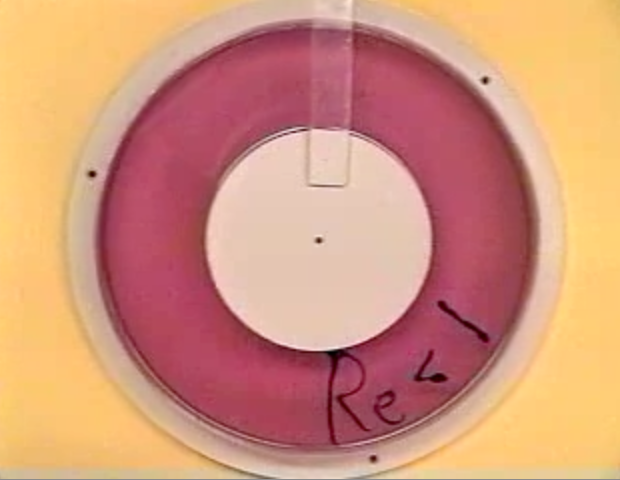
\includegraphics[width=30mm]{kinematic_reverse.png}}{./Figures/kinematic_reverse.mov}}
  		\put(40, 0){\movie[width=30mm,poster,externalviewer,showcontrols=false]{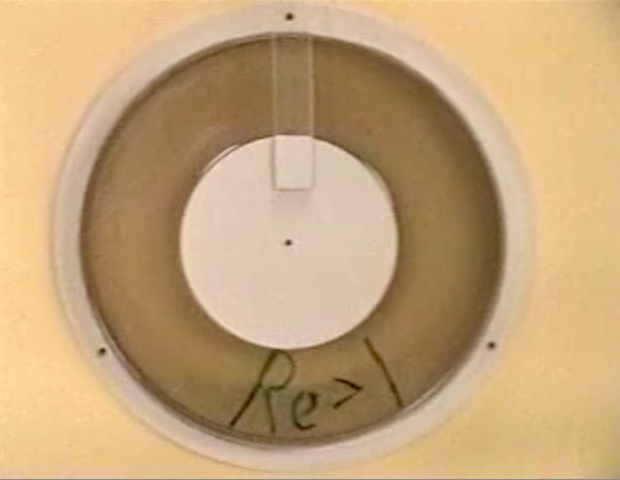
\includegraphics[width=30mm]{kinematic_irreverse.png}}{./Figures/kinematic_irreverse.mov}}
	\end{picture}
\end{center}

\medskip \pause
\item
Le terme non linéaire $(\myvec{u} \cdot \gradient) \myvec{u}$
de l'équation initiale de Navier--Stokes a disparu : 
l'équation de Stokes est une équation \textsl{linéaire}.
$\rightarrow$ \textcolor{vert}{additivité des solutions} à conditions limites différentes.

\medskip \pause
\item
Une autre conséquence est qu'à conditions aux limites données, 
l'équation de Stokes admet une \textcolor{vert}{solution unique}, contrairement au cas général à $Re$ quelconque, 
où la non linéarité des équations autorise l'existence simultanée de plusieurs écoulements solutions.

\end{enumerate}

\vspace{5mm}

\end{frame}

%-----------------------------------------------------------------------------------------
\subsubsection{Solutions}
%-----------------------------------------------------------------------------------------
\begin{frame}{Solutions de l'équation de Stokes}
%-----------------------------------------------------------------------------------------

\small

Bien que plus simple en principe à résoudre que l'équation non linéaire de Navier--Stokes,
l'équation de Stokes reste en pratique délicate à résoudre techniquement, 
même pour des géométries simples d'écoulements. 


\vspace{50mm}

\end{frame}

%-----------------------------------------------------------------------------------------
\begin{frame}{Ecoulements externes : écoulement autour d'une sphère}
%-----------------------------------------------------------------------------------------

\small

%\hspace{-mm}
\begin{minipage}{47mm}
Exemple d'écoulement visqueux autour d'un obstacle :
Solution de Stokes dans le voisinage d'une sphère solide.

\medskip

Cette solution est donnée par

\begin{eqnarray*}
  u_{r} & = & U \cos \theta \left ( 1 - \frac{3a}{2r} + \frac{a^3}{2r^3} \right ) 
  \\
  u_{\theta} & = & -U\sin \theta \left (1 - \frac{3a}{4r} - \frac{a^3}{4r^3} \right )
  \\
  p & = & p_{\infty} - \frac{3}{2} \mu U a \frac{\cos \theta}{r^2}
\end{eqnarray*}
\end{minipage}

\begin{picture}(0, 0)(-51, -2)
	\put( 0,  0){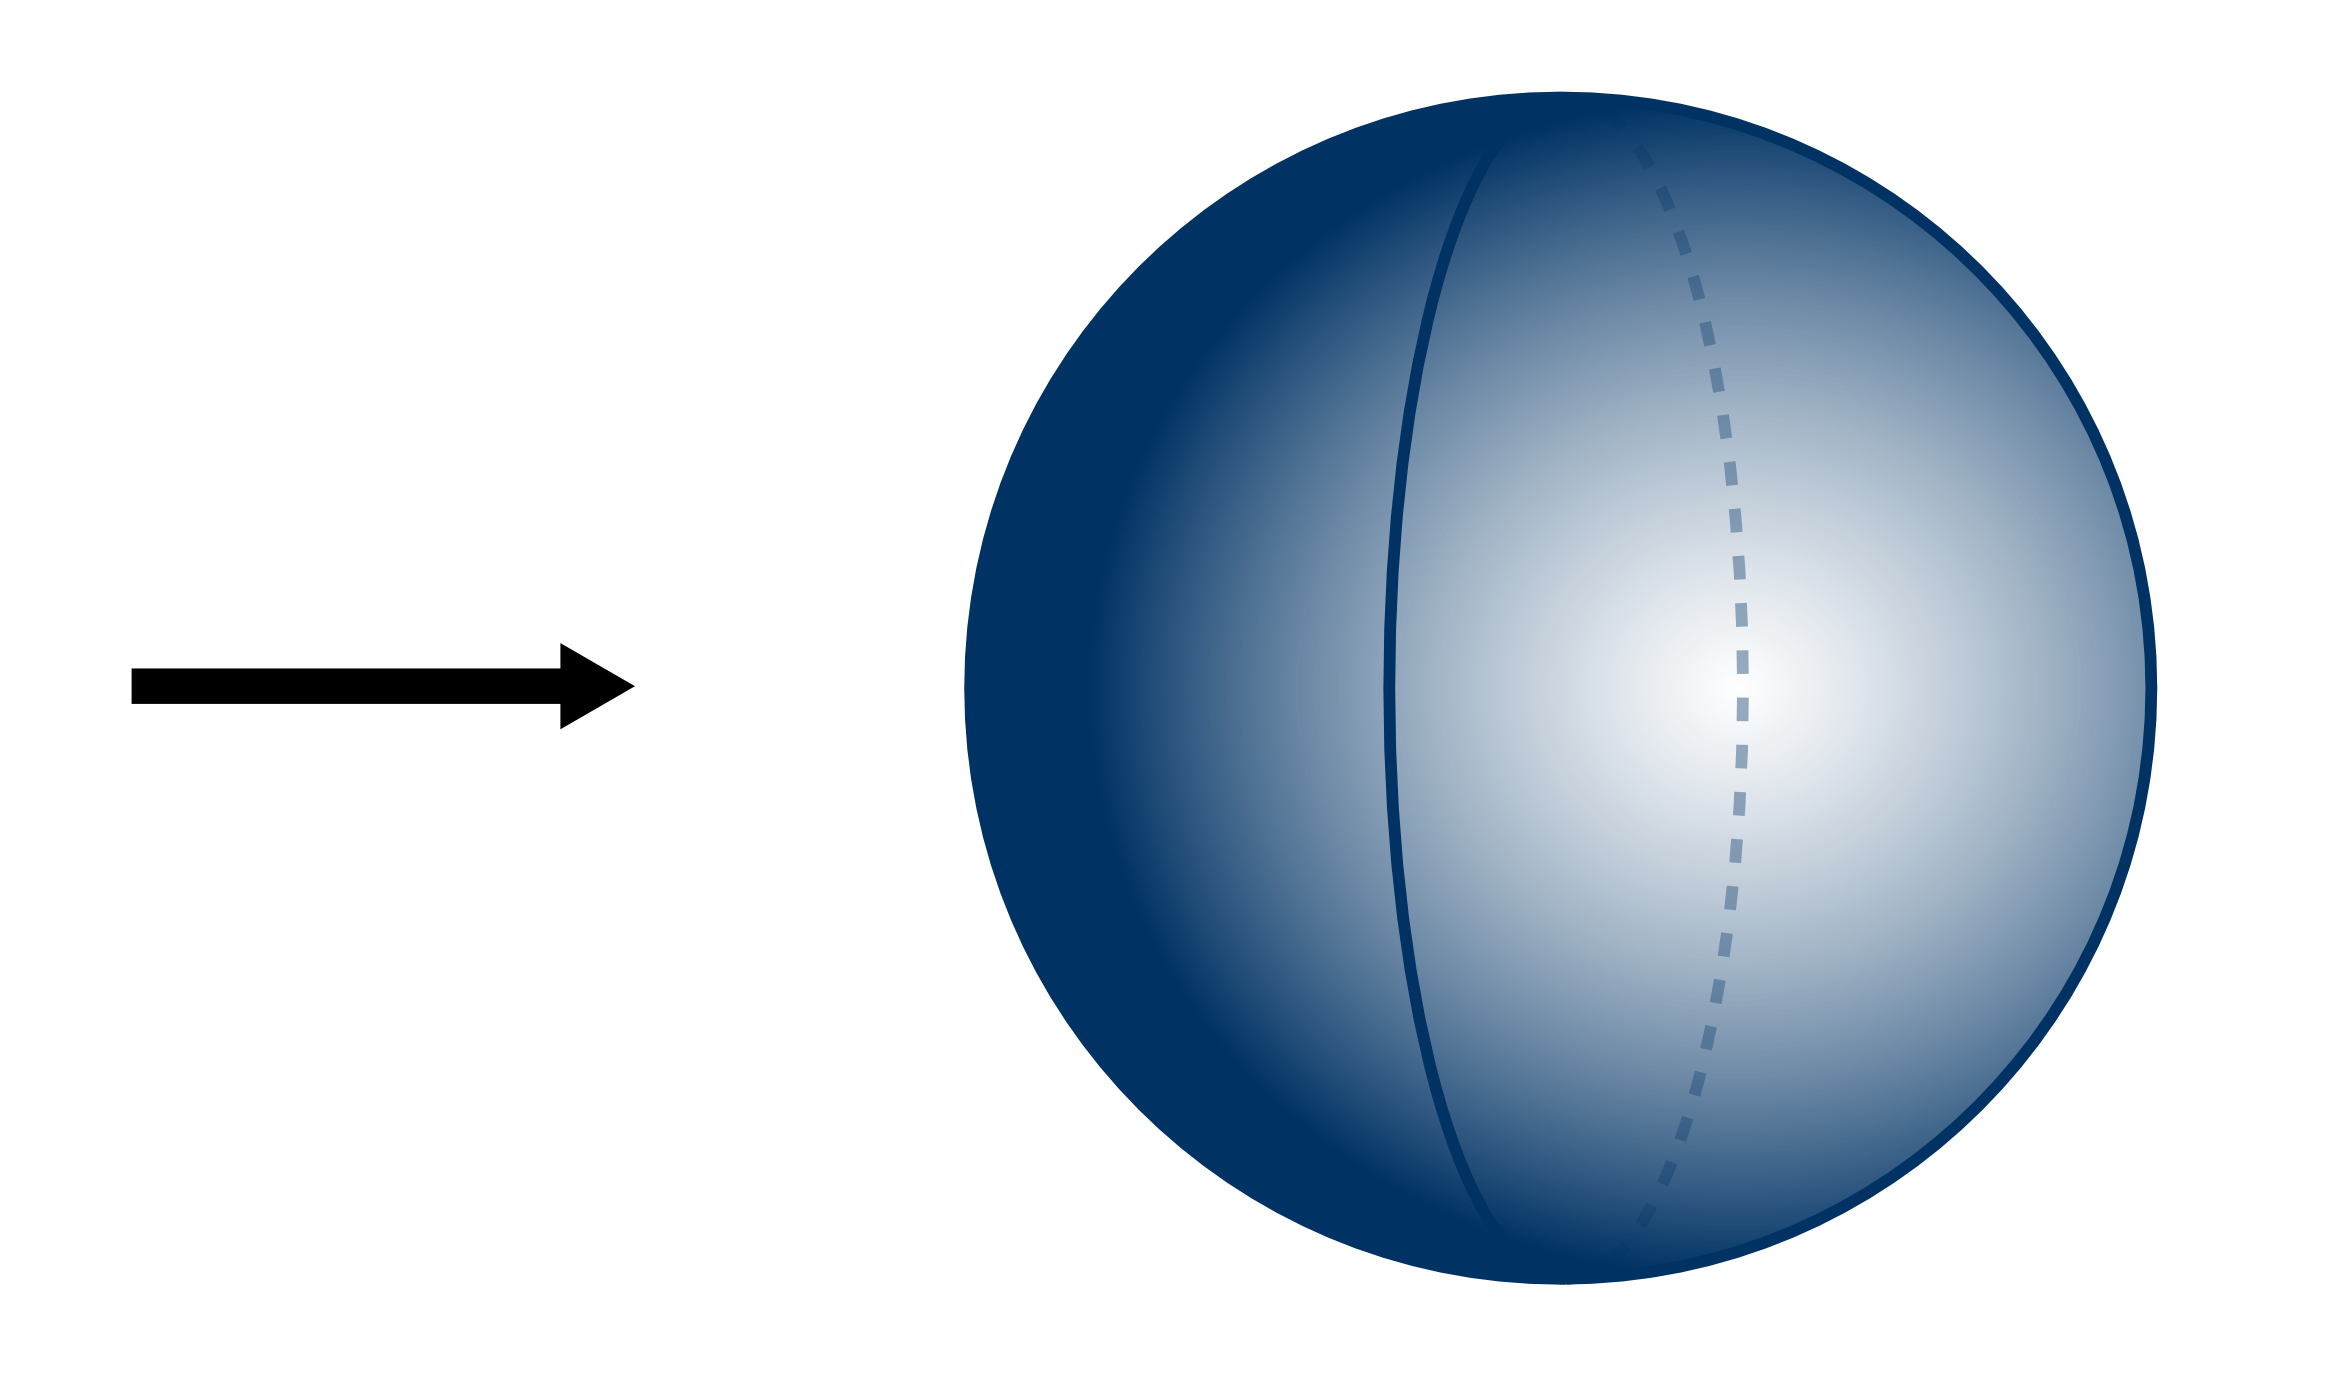
\includegraphics[width=60mm]{sphere.png}}	
	\put( 1, 22){$U, p_\infty$}
	\put(24,  0){\colorbox{white}{$2a$}}
	\put(61, 16.8){$x$}
	\put(25.8, 36){$y$}
	\put(12,  1){$z$}
	\put(53,  13.5){$\varphi$}
	\put(43, 20){$\theta$}
	\put(36.5, 21.8){\setlength{\fboxsep}{0.5mm}\rotatebox{30}{\colorbox{white}{$r$}}}
	\put(54, 30.5){$\myvec{e}_r$}
	\put(37.5, 36){$\myvec{e}_\theta$}
	\put(43.4, 25.1){$\bullet$}
	\put(25.7, 16.5){$\bullet$}
\end{picture}

\bigskip

\textcolor{vert}{Exercice :} Vérifier que cet écoulement est effectivement solution de l'équation
de Stokes en coordonnées sphériques.


\vspace{20mm}

\end{frame}
%-----------------------------------------------------------------------------------------
\begin{frame}{Ecoulements externes : écoulement autour d'une sphère}
%-----------------------------------------------------------------------------------------

\small

Lignes de courant :
\begin{center}
	\begin{picture}(40, 35)(0, 0)
		\put(0, 0){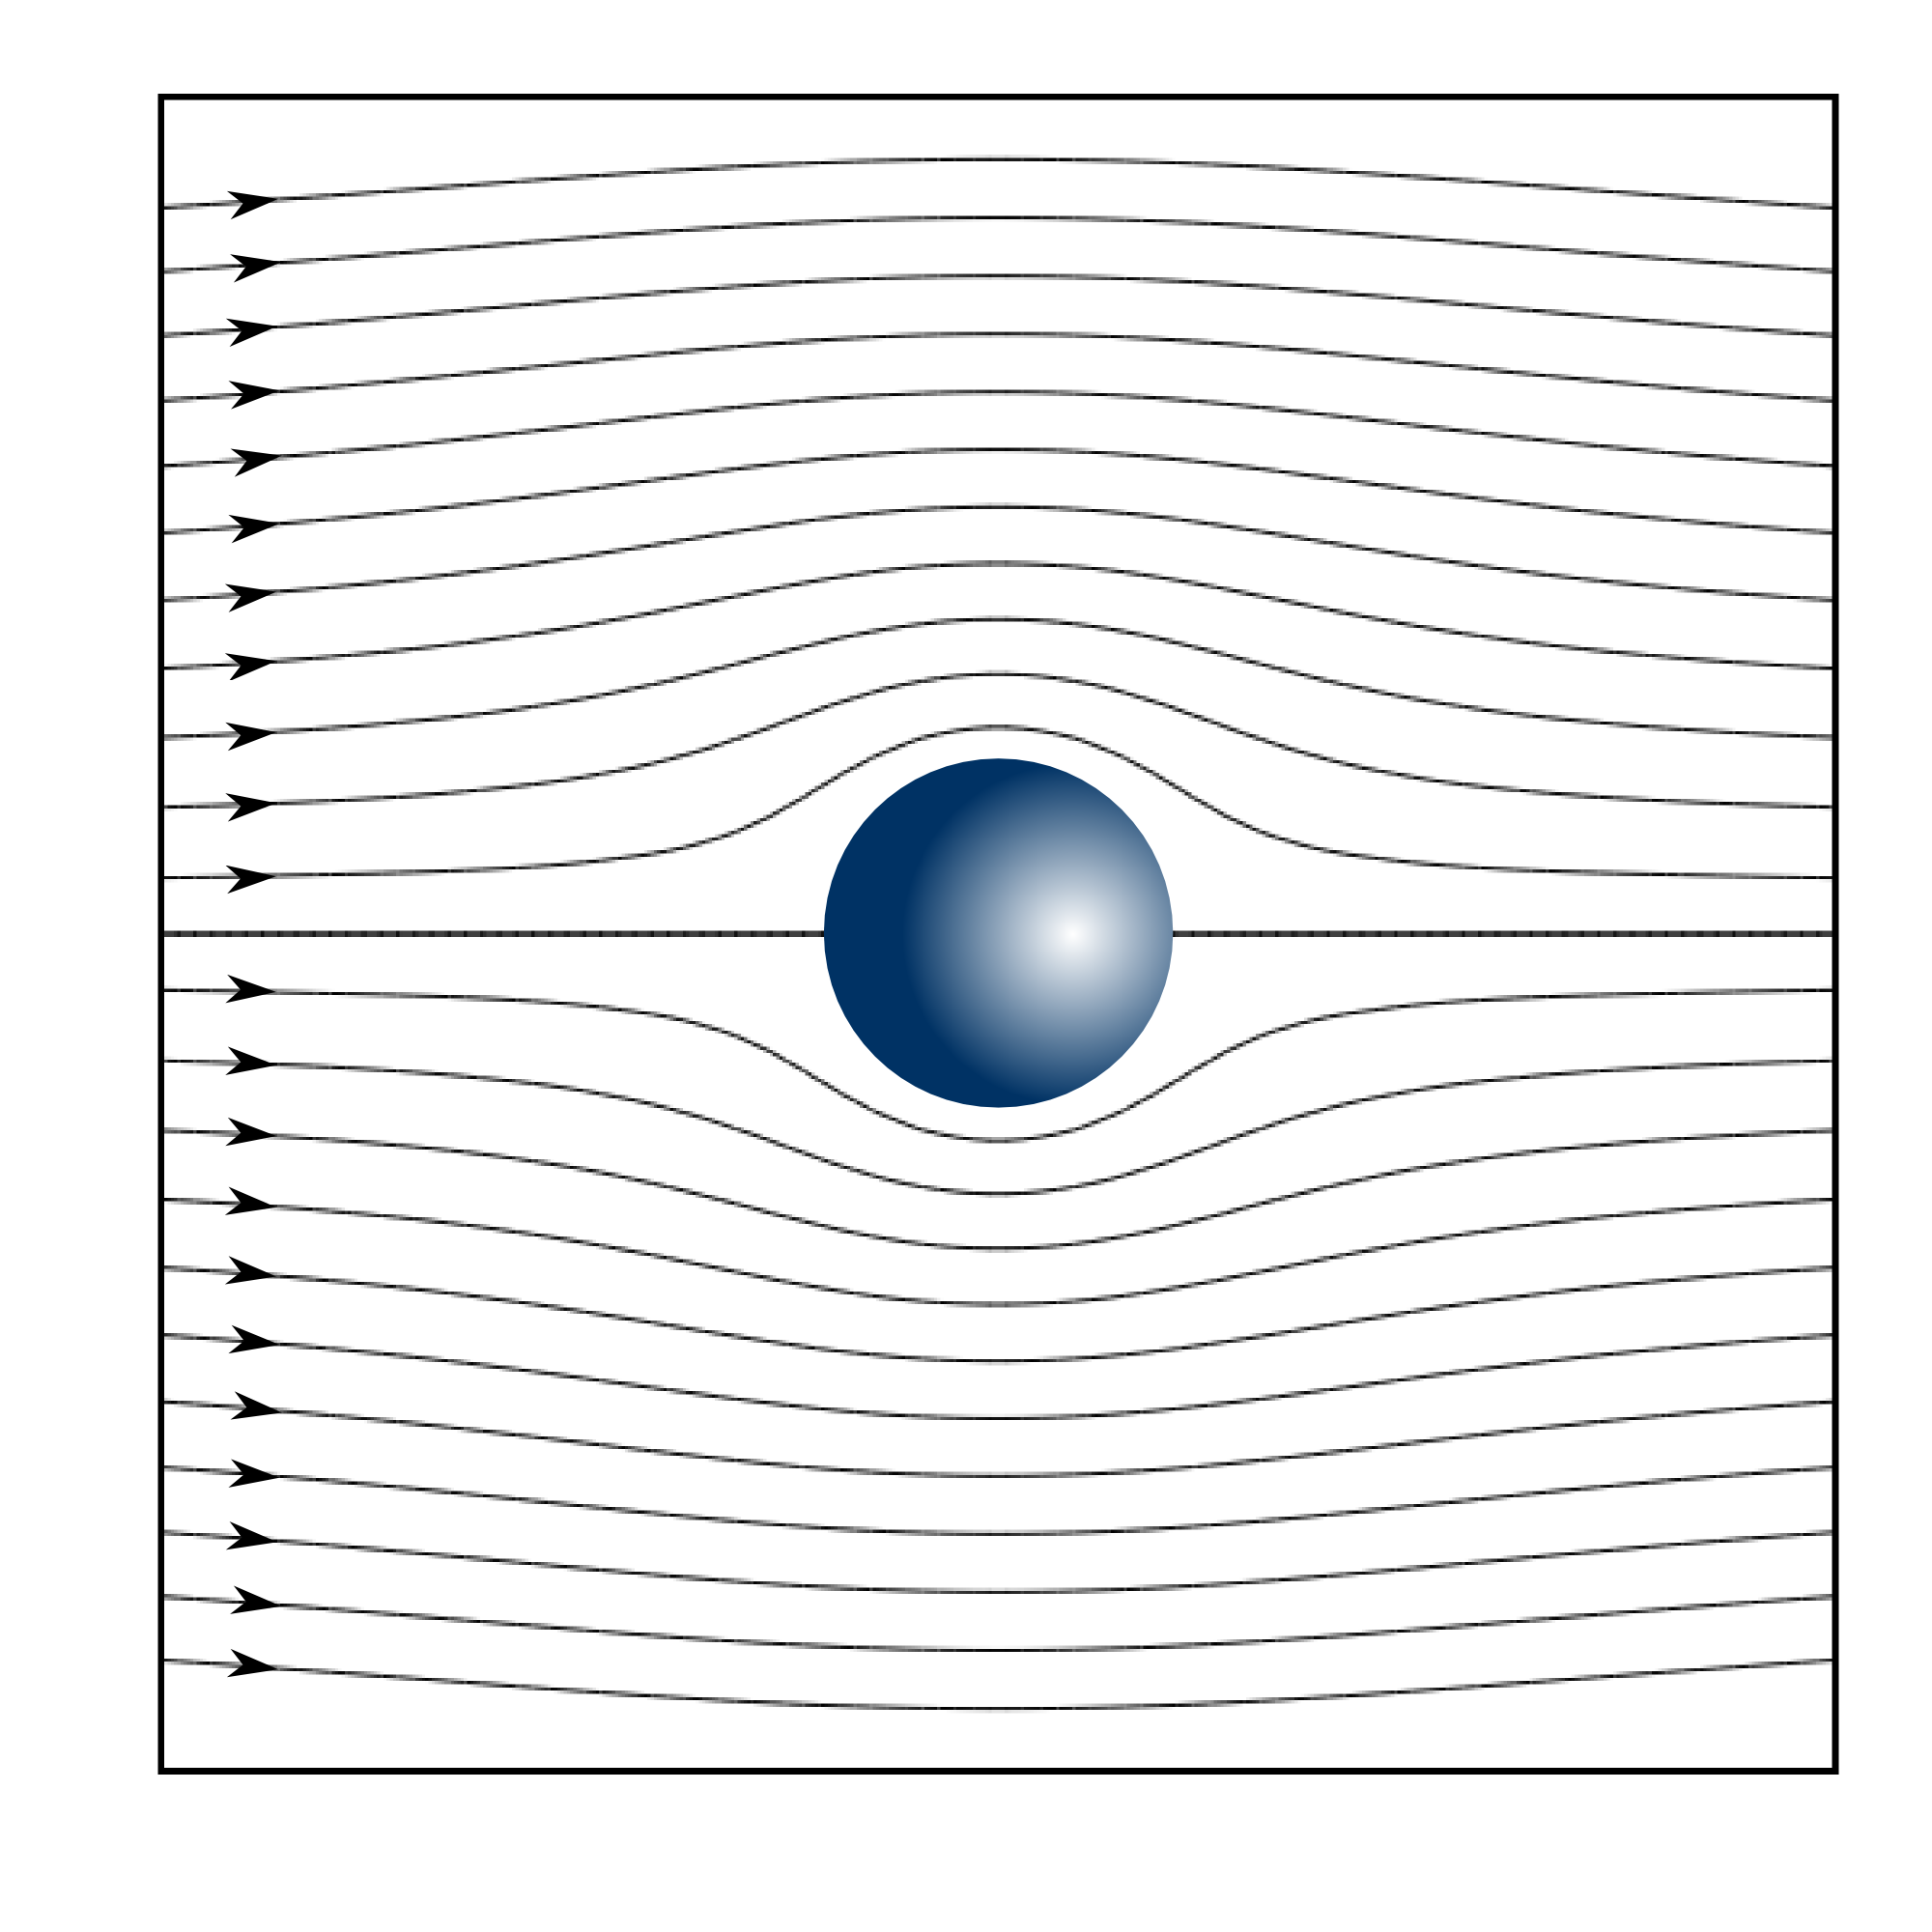
\includegraphics[width=40mm]{streamlines_sphere.png}}	
	\end{picture}
\end{center}

\pause

\textcolor{vert}{Exercice :} on en déduit la force exercée par l'écoulement sur la sphère (\textcolor{vert}{force de Stokes}):
\begin{equation}
  \myvec{F} 
  \equiv 
  \oint_{\mbox{\rm \scriptsize \sl sphère}}
  \mytensor{\sigma} \cdot \myvec{n} \; dS
  =
  \int_{\theta=0}^{\pi} \int_{\varphi=0}^{2\pi} 
  \mytensor{\sigma} \cdot \myvec{e}_{r} \; dS
  =
  \color{rouge} 6\pi \mu U a \, \myvec{e}_{x}
\end{equation}

\textcolor{gris}{Indication : en coordonnées sphériques les composantes nécessaires du tenseur des contraintes visqueuses sont}

$$
\color{gris}{\tau_{rr} = 2 \mu \left( \frac{\partial u_r}{\partial r} \right) ;
\quad   
\tau_{r\theta} = \mu  \left( \frac{1}{r} \frac{\partial u_r}{\partial \theta} 
+ \frac{\partial u_\theta}{\partial r} - \frac{u_\theta}{r} \right) 
}$$

\end{frame}

%-----------------------------------------------------------------------------------------
\begin{frame}{Ecoulements externes : cas général}
%-----------------------------------------------------------------------------------------

\small


Pour des obstacles de forme générale, d'échelle de longueur
caractéristique donnée $L$, 
\\
une estimation de l'ordre de grandeur de la force
exercée par l'écoulement,
\\ \pause
avec des fluctuations de \textcolor{bleu}{pression} d'ordre
\\
\hspace{60mm} \textcolor{bleu}{$[p'] \sim \mu U / L$ }
\\  \pause
et des contraintes de \textcolor{vert}{frottements visqueux} 
d'ordre 
\\
\hspace{60mm} \textcolor{vert}{$\tau \sim \mu U / L$}
\\  \pause
conduit à une résultante 
d'ordre 
\\
\hspace{60mm} $\mu U / L \times L^2$

\bigskip
\pause
soit la force de Stokes générale 
\\
\hspace{60mm} \textcolor{rouge}{$F \sim \mu U L$}
\\
en cohérence avec les résultats exacts précédents.

\begin{center}
	\begin{picture}(40, 30)(0, 0)
		\put(0, 0){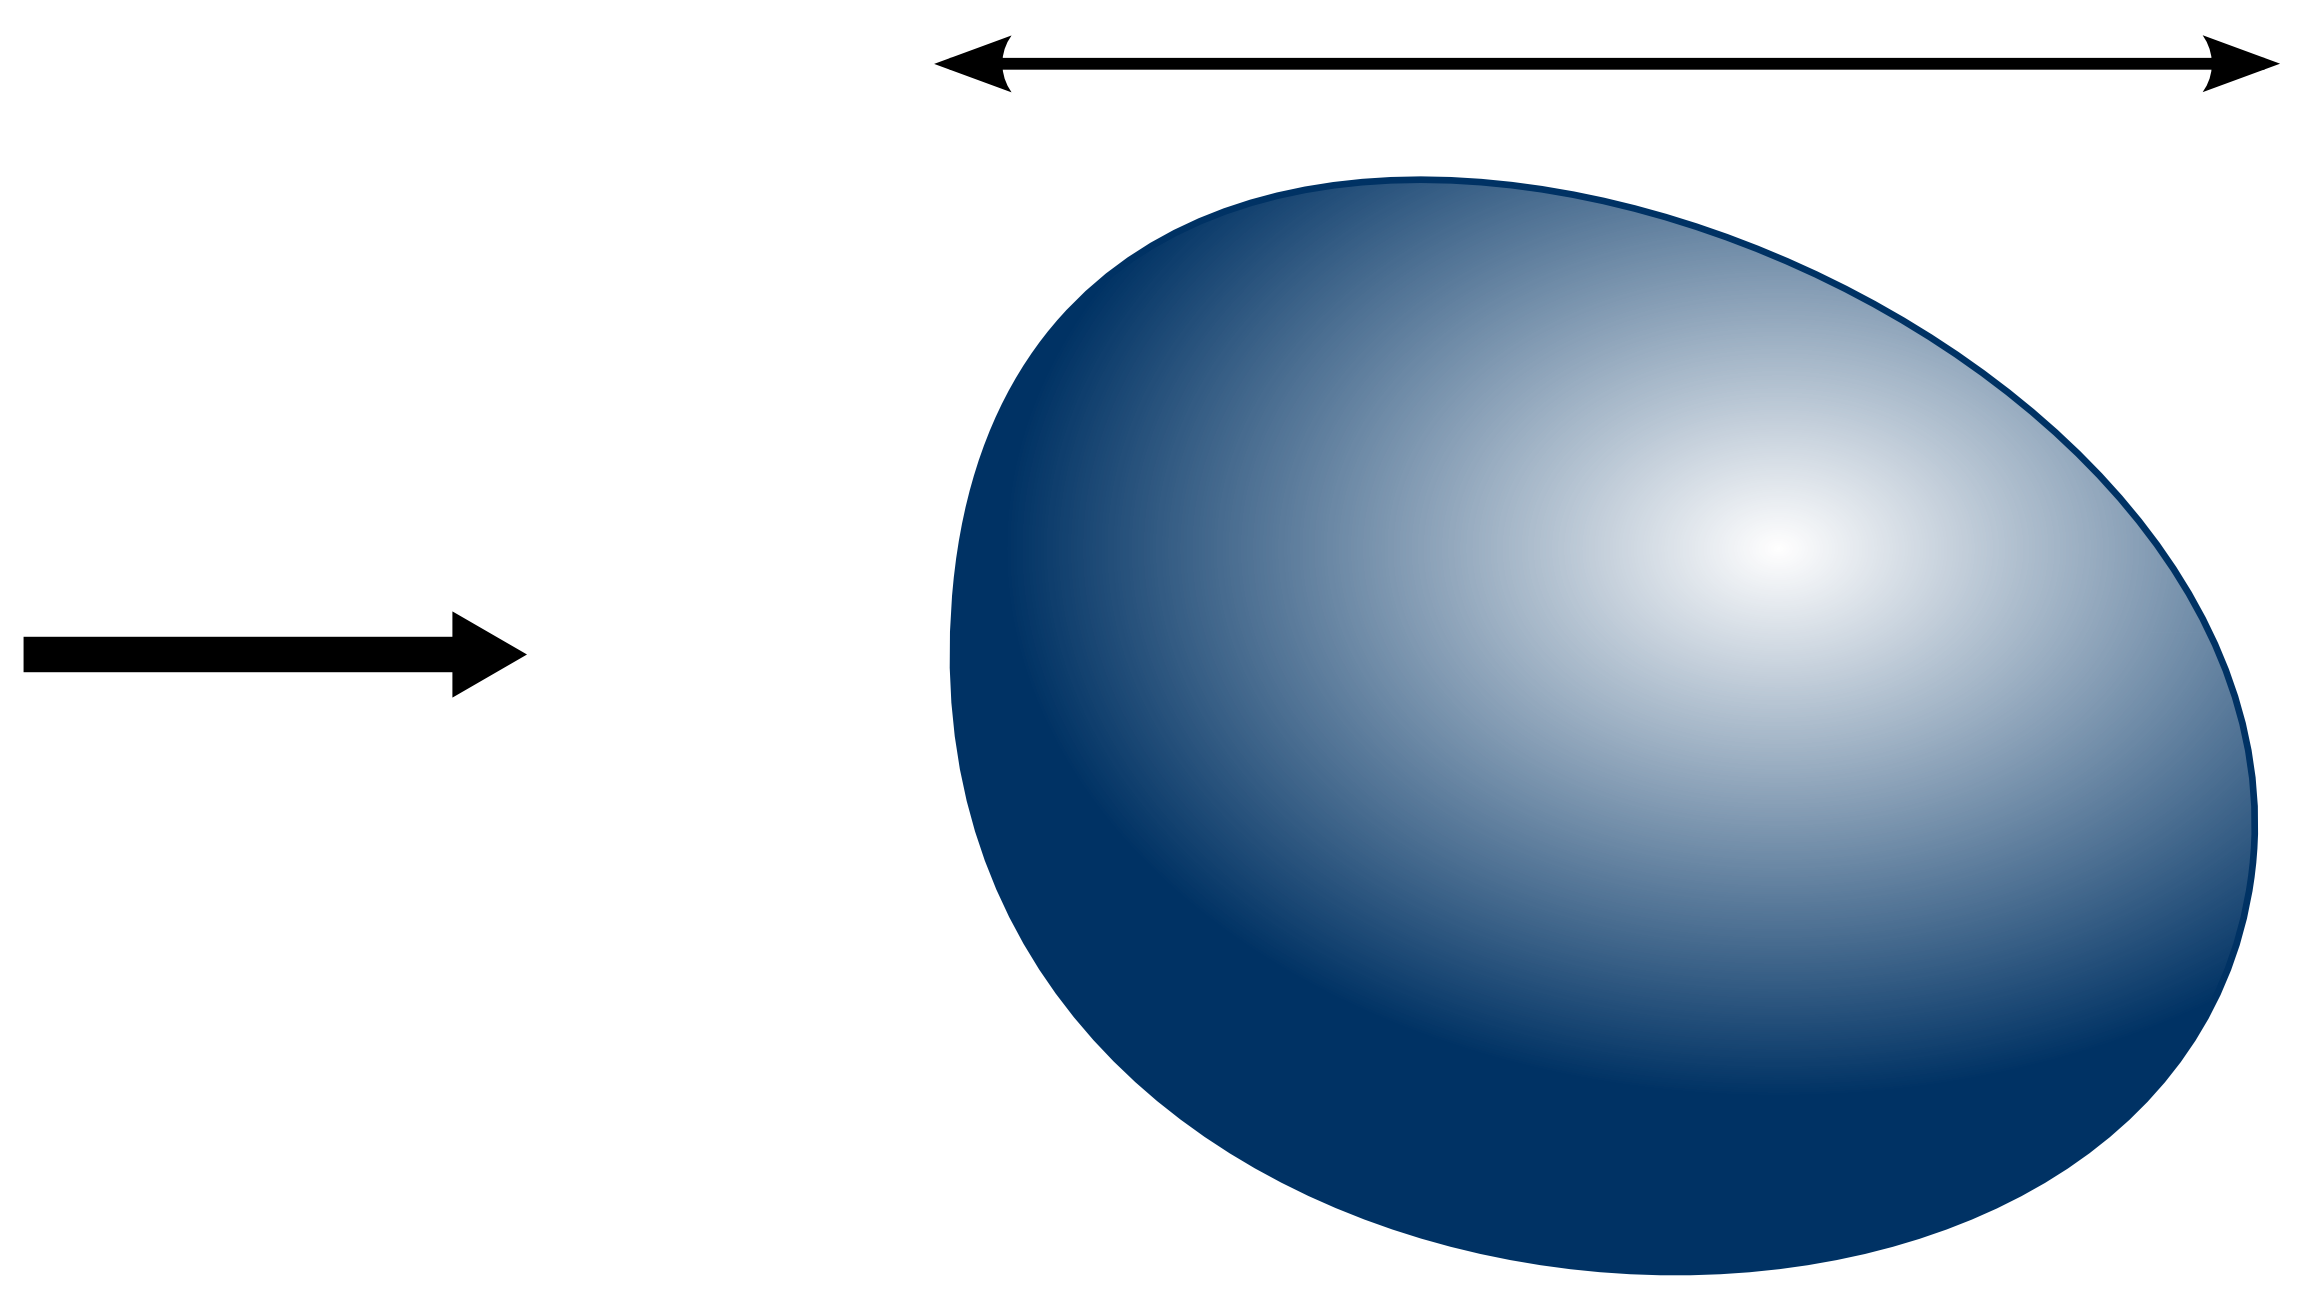
\includegraphics[width=40mm]{obstacle.png}}	
		\put(3, 13){$U$}
		\put(25, 21){\setlength{\fboxsep}{0.5mm}\colorbox{white}{$L$}}
		\put(27, 10){\color{rouge}\vector(1, 0){20}}
		\put(49, 9.5){\color{rouge}$F \sim \mu L U$}
	\end{picture}
\end{center}

\vspace{0mm}

\end{frame}


%-----------------------------------------------------------------------------------------
\begin{frame}{Ecoulements autours d'obstacles}
%-----------------------------------------------------------------------------------------



Outre la sphère, il existe très peu de cas où l'écoulement (et la force correspondante)
ont des expressions analytiques.
\medskip

Quelques exemples :

\medskip
\begin{itemize}

\item
Bulle sphérique de rayon $a$ :

$ \color{rouge} 
  \myvec{F} 
  =
  4\pi \mu U a \, \myvec{e}_{x}
$

(géométrie identique à une sphère mais conditions limites en $r=a$ différentes !)

\vspace{0mm}

\medskip 
\item Disque de rayon $a$ et d'épaisseur nulle (axe aligné avec l'écoulement) : %(placé perpendiculairement à l'écoulement) : 

$ \color{rouge} 
  \myvec{F} 
  =
  16 \mu U a \, \myvec{e}_{x}  
$

\medskip 
\item Disque de rayon $a$ et d'épaisseur nulle (axe perpendiculaire à l'écoulement) :

$ \color{rouge} 
 \myvec{F} 
  =
  \frac{32}{3}  \mu U a \, \myvec{e}_{x}
$
\medskip


\item Cylindre de rayon $a$ et de longueur $L$ (axe perpendiculaire à l'écoulement) :
$ \color{rouge} 
  \myvec{F} 
  \approx \mu U a \log \left( \frac{L}{a} \right)   \myvec{e}_{x}
$
\end{itemize}

\medskip

Remarque : pour un cylindre de longueur infinie ($L/a \rightarrow \infty$) 

Il n'existe pas de solution à l'équation de Stokes en 2 dimensions !

(Paradoxe de Stokes )

\end{frame}


%-----------------------------------------------------------------------------------------
\begin{frame}{Ecoulements internes}
%-----------------------------------------------------------------------------------------

\small

Il n'existe pas de solution générale de Stokes dans des conduites ou canaux.

\medskip \pause

On peut cependant remarquer (exercice) que toute solution stationnaire de l'équation de Navier--Stokes vérifiant 
\[
	\color{rouge}
	(\myvec{u} \cdot \gradient) \myvec{u} = \myvec{0}
\]

est automatiquement solution exacte de Stokes.

\pause
\bigskip

C'est en particulier (exercice) le cas des écoulements dits \textcolor{vert}{parallèles},
de la forme
\[
	\myvec{u} = u(y)\; \myvec{e}_{x} \quad \mbox{(en géométrie cartésienne)}
\]
ou 
\[
	\myvec{u} = u(r)\; \myvec{e}_{x}  \quad \mbox{(en géométrie cylindrique)}
\]

\medskip
On en déduit que les écoulements de Poiseuille plan et cylindrique, de film
tombant, de Couette plan avec ou sans gradient de pression sont solutions exactes de l'équation de Stokes.

\medskip
\pause

S'il n'existe pas de solution simple si l'écoulement n'est pas parallèle, on peut cependant chercher des solutions approchées dans le cas des écoulements 
\textcolor{vert}{quasi-parallèles} (cf. section suivante).


\vspace{15mm}

\end{frame}

%==========================================================================================
\subsection{Les écoulements de films minces}
%=========================================================================================

%-----------------------------------------------------------------------------------------
\subsubsection{Définition}
%-----------------------------------------------------------------------------------------
\begin{frame}{Définition}
%-----------------------------------------------------------------------------------------

\small

On appellera \textcolor{rouge}{film mince} tout écoulement de fluide dont l'épaisseur caractéristique 
$|e(x, t)| \sim \delta$ est faible comparée à l'échelle 
caractéristique de variation longitudinale $L$ :
\[
	\delta \ll L \quad \Rightarrow \quad \varepsilon = \frac{\delta}{L} \ll 1
\]

\begin{center}
	\setlength{\unitlength}{1mm}
	\begin{picture}(80, 28)
		\put(0, 0){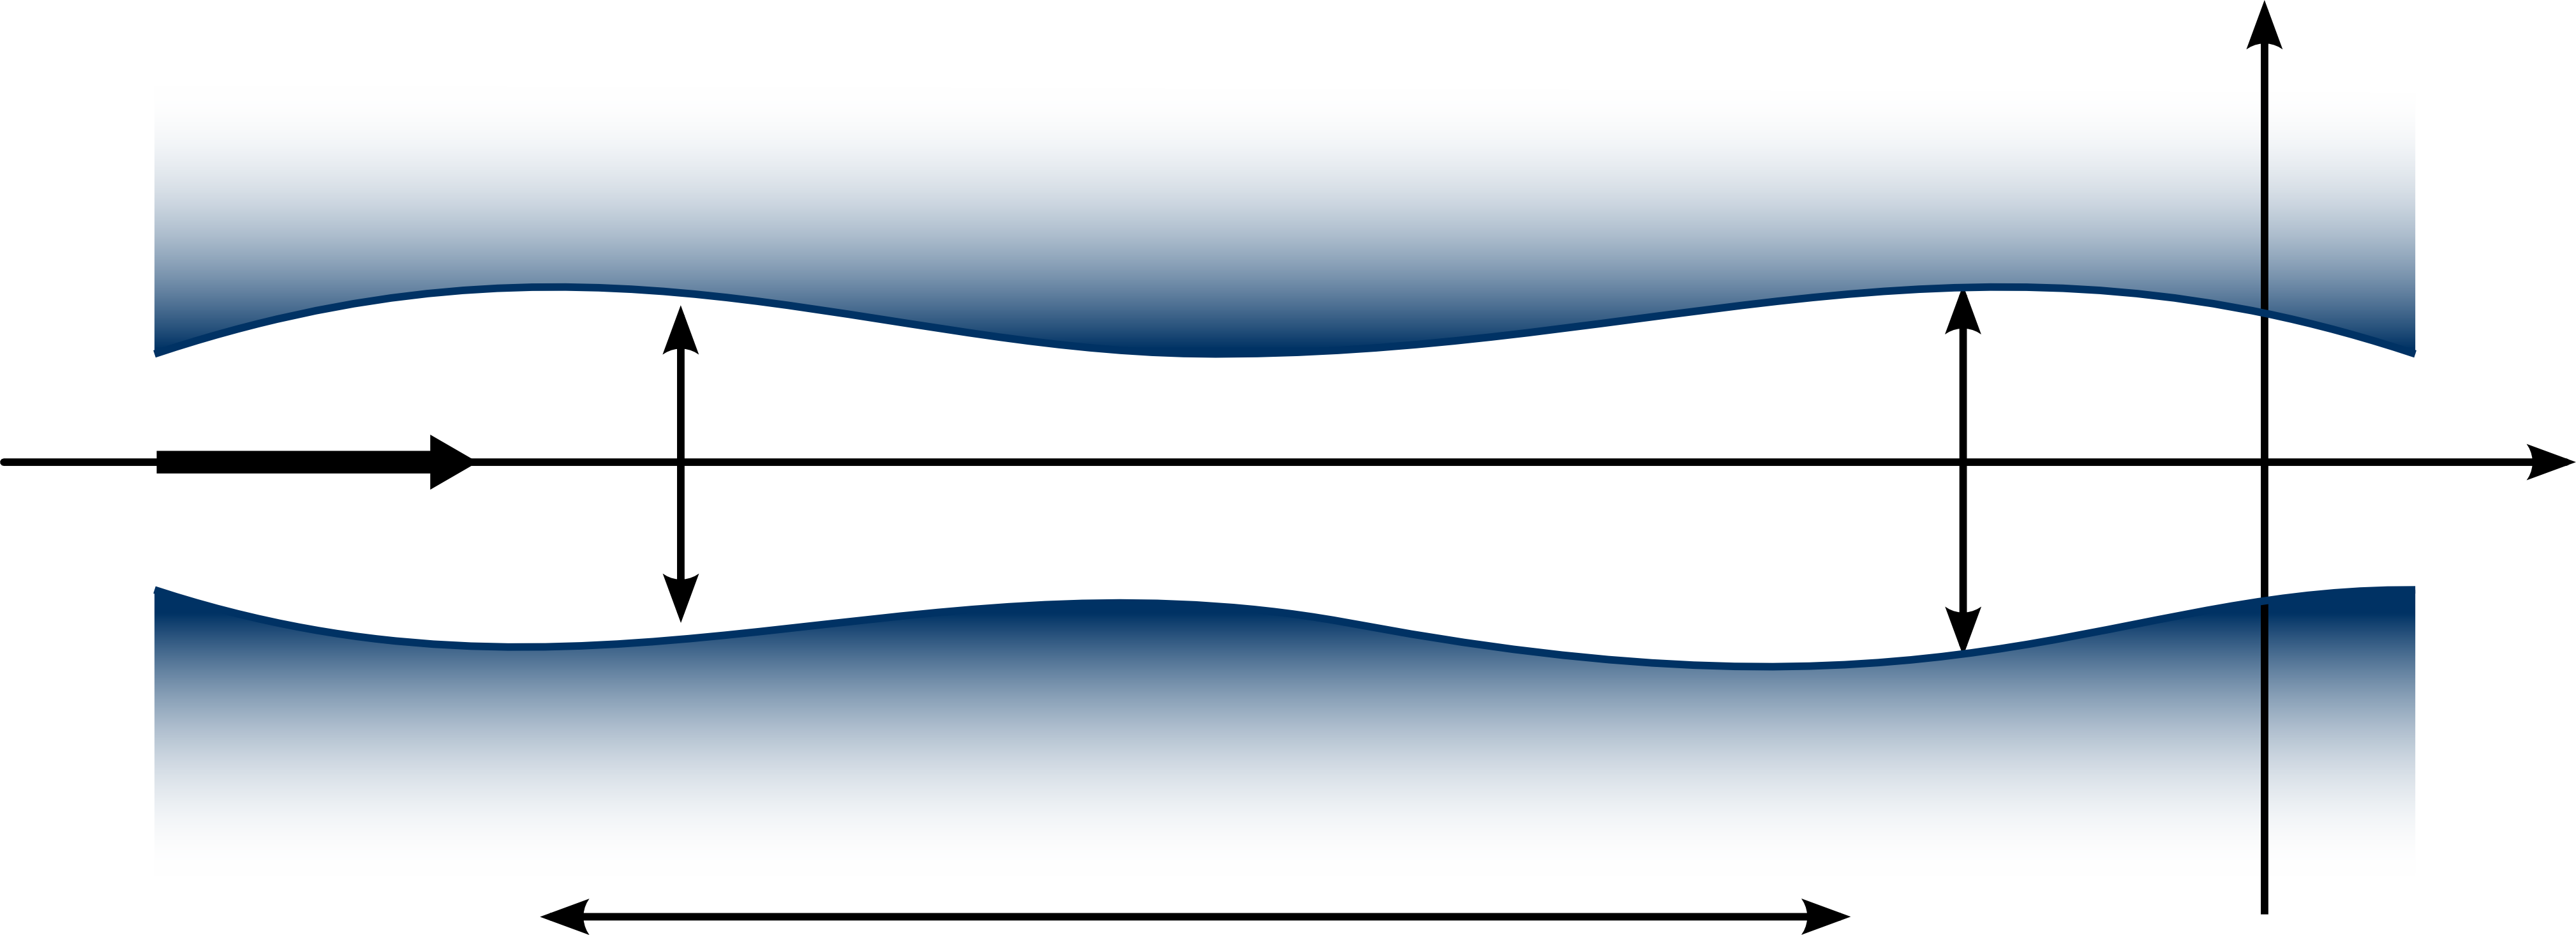
\includegraphics[width=80mm]{film_mince.png}}	
		\put( 8, 16){$\sim U$}
		\put(19, 14){\setlength{\fboxsep}{0.5mm}\colorbox{white}{$\sim \delta$}}
		\put(32,  -0){\setlength{\fboxsep}{0.5mm}\colorbox{white}{$\sim L$}}
		\put(57, 14){\setlength{\fboxsep}{0.5mm}\colorbox{white}{$e(x, t)$}}
		\put(69.5, 30.5){$y$}
		\put(81, 14.2){$x$}
		\put(76, 18.5){$y=h_2(x, t)$}
		\put(76,  9.5){$y=h_1(x, t)$}
		\put(25, 12){$\mbox{\sl \footnotesize \color{bleu} milieu 0 : fluide}$}
		\put(12, 4){$\mbox{\sl \footnotesize \color{bleu} milieu 1 (fluide ou solide, fixe ou mobile)}$}
		\put(12, 24){$\mbox{\sl \footnotesize \color{bleu} milieu 2 (fluide ou solide, fixe ou mobile)}$}
	\end{picture}
\end{center}

\pause
Dans ce cas, l'écoulement est dit \textcolor{rouge}{quasi-parallèle}.

\medskip
\pause
Si $U$ désigne une vitesse caractéristique de l'écoulement, alors on définit classiquement
le nombre de Reynolds du film comme
\[
	Re = \frac{U\delta}{\nu}
\]
où $\nu$ désigne la viscosité cinématique du fluide.

\pause
\medskip

L'étude de la dynamique des films minces est l'objet de la \textcolor{vert}{théorie de la lubrification}.

\vspace{5mm}

\end{frame}

%-----------------------------------------------------------------------------------------
\subsubsection{Equations de film mince}
%-----------------------------------------------------------------------------------------
\begin{frame}{Equations de film mince}
%-----------------------------------------------------------------------------------------

\small

\textbf{Hypothèses et équations de base :} \medskip

Ecoulement plan, incompressible, de fluide homogène ($\rho$ uniforme) et newtonien

\medskip \pause

$\rightarrow \myvec{u} = u(x, y, t) \, \ex + v(x, y, t)\, \ey$

\medskip

avec 
\[
	\divergence \myvec{u} = 0
\] 
et 
\[
	\dpdt{\myvec{u}} +(\myvec{u}\cdot\gradient\ ) \myvec{u} 
	= 
	-\frac{1}{\rho} \gradient p + \myvec{g} + \nu \Delta\myvec{u}
	=
	-\frac{1}{\rho} \gradient \hat{p} + \nu \Delta\myvec{u}	
\]
où $\hat{p} = p + \rho g z$ est la pression motrice.

\bigskip

\pause

D'où les équations scalaires suivantes :
\begin{eqnarray}
	\dpdx{u} + \dpdy{v} 
	\label{eq:continuite}
	& = & 
	0
	\\
	\dpdt{u} + u\dpdx{u} + v\dpdy{u}  
	& = & 
	-\frac{1}{\rho} \dpdx{\hat{p}} + \nu \left ( \ddpdx{u} + \ddpdy{u} \right )
	\label{eq:qdmx}
	\\
	\dpdt{v} + u\dpdx{v} + v\dpdy{v}  
	& = & 
	-\frac{1}{\rho} \dpdy{\hat{p}} + \nu \left ( \ddpdx{v} + \ddpdy{v} \right )
	\label{eq:qdmy}
\end{eqnarray}

\small

\vspace{5mm}

\end{frame}

%-----------------------------------------------------------------------------------------
\begin{frame}{Equations de film mince}
%-----------------------------------------------------------------------------------------

\small

\textbf{Analyse dimensionnelle des équations :} \medskip

Ordres de grandeurs : 

%$\rightarrow$ changement de variables :
%\smallskip


\begin{center}
	\begin{tabular}{lp{3mm}ll}
		$\color{rouge} x = {\mathcal O} (L)$  & & $L$ :  &  échelle caractéristique de longueur suivant $x$
		\\
		$\color{rouge} y =  {\mathcal O} (\delta)$ &  & $\delta$ : & \dotfill\ de longueur suivant $y$
		\\
		$\color{rouge} t =  {\mathcal O} (\tau)$ &  & $\tau$ : & \dotfill\ de temps 		\\
		$\color{rouge} u =  {\mathcal O} (U)$ &  & $U$ : & \dotfill\ de vitesse longitudinale
		\\
		$\color{rouge} v =  {\mathcal O} (V)$ &  & $V$ : & \dotfill\ de vitesse transversale
		\\
		$\color{rouge} \hat{p} =  {\mathcal O} ([p'])$ &  & $[p']$ : & \dotfill\ de (variation de) pression
		
	\end{tabular}
\end{center} 


\smallskip

Les échelles $L,\delta,U,\tau$ sont imposées par les données du problème ; {\tiny (si le problème est stationnaire $\tau=\infty$)}

\smallskip

Les échelles $V$ et $[p']$, ordres de grandeur non connus de vitesse normale et des variations de pression motrice, sont à déterminer par examen des équations en appliquant le principe de moindre dégénerescence (PMD) :

\smallskip

\begin{quotation}
"on simplifie en gardant le maximum de termes possible"
\end{quotation}

\small

%\vspace{5mm}

\end{frame}

%-----------------------------------------------------------------------------------------
\begin{frame}{Equations de film mince}
%-----------------------------------------------------------------------------------------

\small

\textbf{Après simplification asymptotique :} \hfill \textcolor{gris}{[Démonstration]}

\bigskip

\begin{itemize}
\item
	Eq.~(\ref{eq:continuite}) 
	$\quad \Rightarrow \quad \color{rouge} V = \dfrac{\delta}{L} U = \varepsilon \, U$ \quad (PMD)
\item[] d'où
	\begin{equation}
		\color{rouge}
		\dpdx{u} + \dpdy{v} = 0
	\end{equation}
\item
	Eq.~(\ref{eq:qdmx}) $\quad \Rightarrow \quad \color{rouge} [p'] = \mu U \dfrac{L}{\delta^2}$ \quad (PMD)
	
	\quad Si $\color{vert} \frac{\delta^2  U}{\nu L} = \varepsilon Re \ll 1$, le terme d'advection est négligeable,
	
	\quad Si $\color{vert} \frac{\tau}{\tau_d} = \tau \frac{ \nu}{L^2} \gg 1$, le terme de dérivée temporelle est négligeable,
	
\item[] d'où
	\begin{equation}
		\color{rouge}
		-\dpdx{\hat{p}} + \mu \ddpdy{u} = 0
	\end{equation}
\item
	Finalement Eq.~(\ref{eq:qdmy}) se réduit à
	\begin{equation}
		{\color{rouge}
		\dpdy{\hat{p}} = 0},
		\quad \mbox{soit} \quad \color{rouge}\hat{p} = \hat{p}(x, t)
	\end{equation}
\end{itemize}


\small

\vspace{10mm}

\end{frame}

%-----------------------------------------------------------------------------------------
\subsubsection{Solution générale de film mince}
%-----------------------------------------------------------------------------------------
\begin{frame}{Solution générale de film mince}
%-----------------------------------------------------------------------------------------

\small

On en déduit la solution générale : \hfill \textcolor{gris}{[Démonstration]}
\begin{eqnarray*}
	\left .
	\begin{array}{r}
		-\dpdx{\hat{p}} + \mu \ddpdy{u} = 0
		\\ \\
		\hat{p} = \hat{p}(x, t) 
	\end{array}
	\right \}
	& \Rightarrow & \ddpdy{u} = \dfrac{1}{\mu} \dpdx{\hat{p}}(x, t)
	\\
	& \Rightarrow & 
	\color{rouge}
	u(x, y, t) = \dfrac{1}{2\mu} \dpdx{\hat{p}}(x, t) y^2 + A(x, t) y + B(x, t)
\end{eqnarray*}
où $A(x, t)$ et $B(x, t)$ sont à déterminer à l'aide des conditions aux limites avec les milieux 1 et 2
en $y=h_1(x, t)$ et $y=h_2(x, t)$.

\bigskip
\pause

De plus :
\begin{eqnarray*}
	\dpdx{u} + \dpdy{v} = 0 
	& \Rightarrow &
	\dpdy{v} = - \dpdx{u} = -\dfrac{1}{2\mu} \ddpdx{\hat{p}}(x, t) y^2 - \dpdx{A}(x, t) y - \dpdx{B}(x, t)
	\\
	& \Rightarrow & \color{rouge}
	v(x, y, t) = -\dfrac{1}{6\mu} \ddpdx{\hat{p}}(x, t) y^3 
	             - \dfrac{1}{2}\dpdx{A}(x, t) y^2 - \dpdx{B}(x, t)	y + C(x, t)
\end{eqnarray*}
où $C(x, t)$ est à déterminer à l'aide des conditions aux limites.

\vspace{5mm}

\end{frame}

\begin{frame}{Exemple d'application : écoulement entre deux cylindres}

\small

Considérons l'écoulement à travers l'étranglement entre deux cylindres de rayon $R$, longueur $L$, séparés par une distance $\delta \ll R$. 

\smallskip 
Dans ce cas : 

$
e(x) = \delta + 2 (R- \sqrt{ R^2- x^2}) %\approx \delta + x^2/R
$

\smallskip 
\textcolor{green}{Problème :} déterminer la relation entre $Q_m$ (débit massique) et $\Delta P$ (variation de pression a travers l'étranglement)  

\pause 

\bigskip
Solution (exercice) : 
$$
u(x,y) = \frac{1}{2\mu} \dpdx{p} (y^2- (e(x)/2)^2)  
$$

$$
Q_m  = \rho L \int_{-e(x)/2}^{+e(x)/2} u(x,y) d y =  - \frac{\rho L}{12 \mu}  e(x)^3 \dpdx{p}
$$

$$
\Delta P = \int_{-R}^{+R}  \dpdx{p} dx  =  - \frac{12 \mu Q_m}{\rho L} \int_{-R}^{+R} \frac{1}{e(x)^3} dx
$$

L'intégrale peut être évaluée et a l'expression suivante :

$$ 
\int_{-R}^{+R} \frac{1}{(\delta + 2 R- 2 \sqrt{ R^2- x^2}) ^3} dx \approx \frac{3\pi}{8} \sqrt{\frac{R}{\delta^5}}
$$

Finalement :

$$
\Delta P = - \frac{9 \pi}{2} \frac{\mu Q_m}{\rho L} \sqrt{\frac{R}{\delta^5}}
$$



\end{frame}


\comment{
%==========================================================================================
\subsection*{Compléments}
%==========================================================================================

%------------------------------------------------------------------------------------------
\begin{frame}{Quelques solutions exactes} \hypertarget{frame:toto}{}
%------------------------------------------------------------------------------------------

\begin{center}
	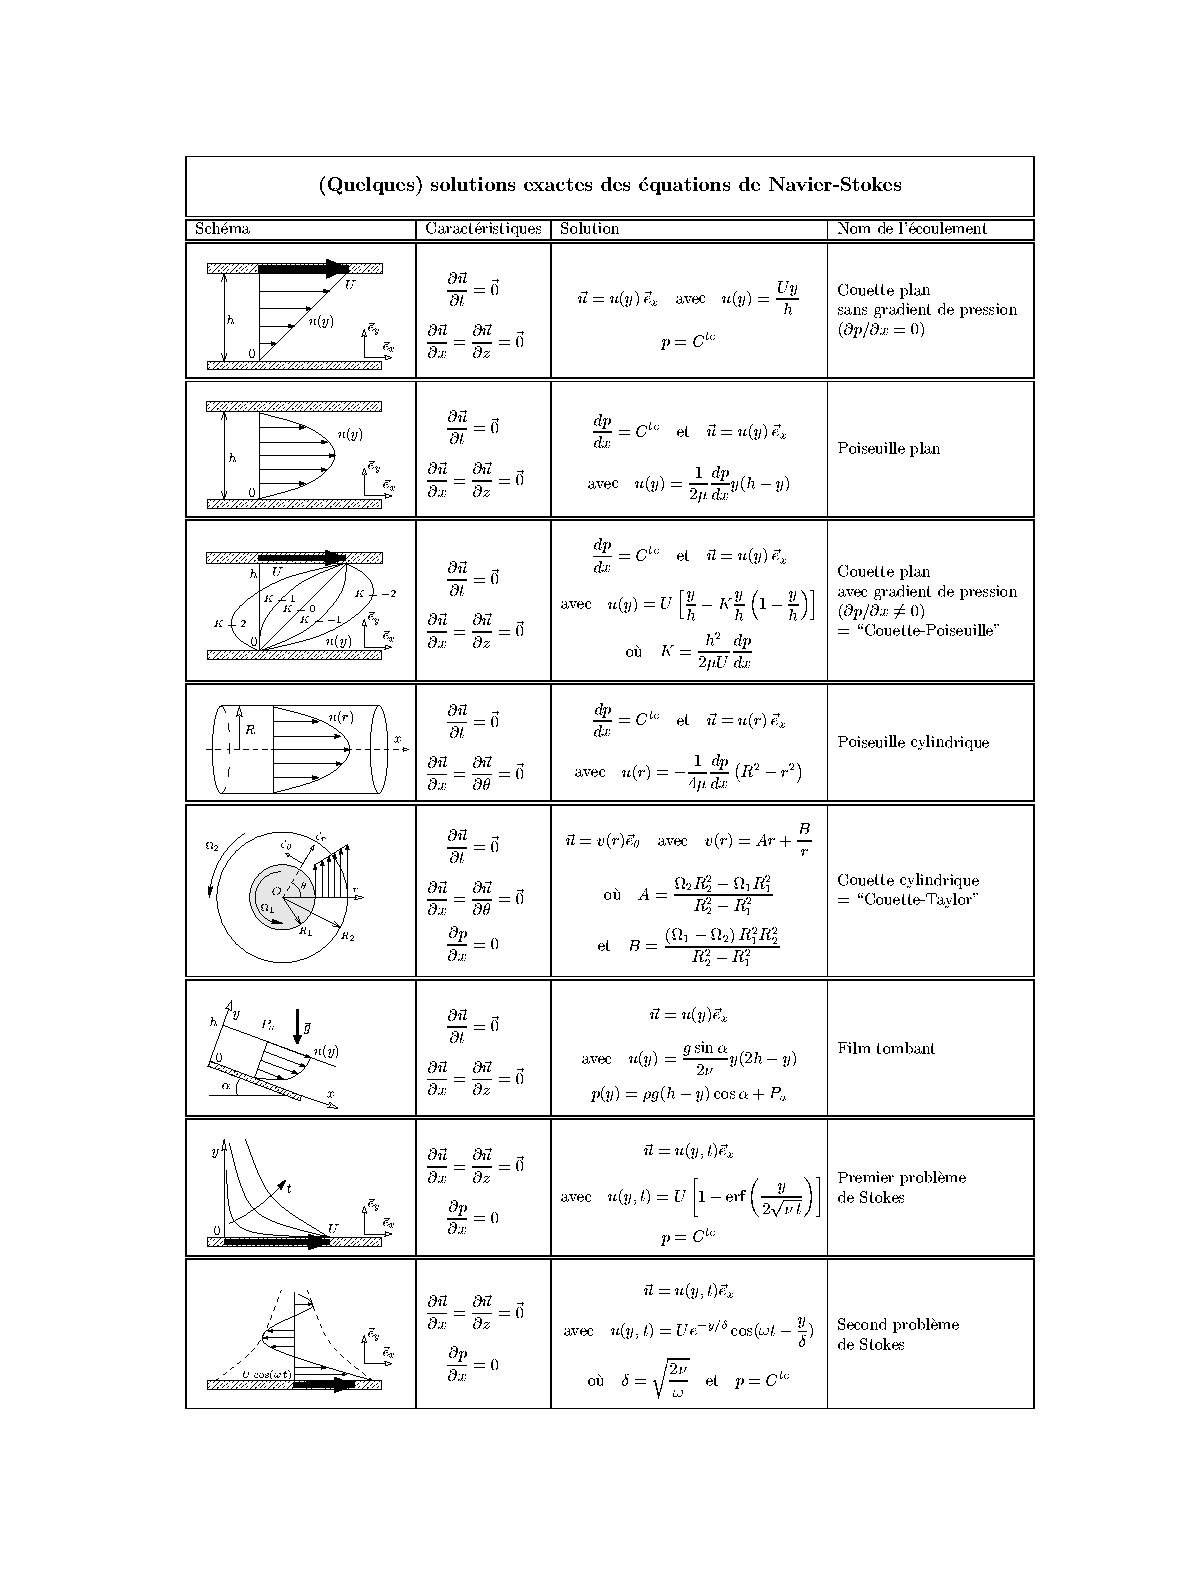
\includegraphics[height=.8\linewidth]{solutions_exactes}
\end{center}

%\vspace{0mm}
\end{frame}
}

\end{frame}

